\section{Introduction}
\label{sec:intro}

Data exploration is the act of querying a database to discover its content.
Ultimately, the aim is to discover \emph{nuggets}, i.e., interesting queries
that expose unexpected phenomena.  Because this task
is important and omnipresent, engineers have devised \emph{exploration
systems} to support it. These systems let users ``play'' with their tuples. They
provide facilities to write queries and visualize the results quickly.
They engage their users in a loop of trial and errors, through which they discover
their data. Examples of such systems are Tableau~\cite{StolteTangHanrahan2002},
based on visualizations, BlinkDB~\cite{agarwal2012blink}, based on sampling, or
Blaeu~\cite{sellamTKDE} based on clustering.

Exploration systems assume that users can evaluate the usefulness of a set of
tuples simply by looking at it - or at least, by looking at a sample.
Typically, they present the results of the queries with tables, visualizations,
or statistical summaries, in the hope that users will know what to inspect and
where to go next. And indeed, this assumption holds with low dimension data.
If a set of tuples involves less than a dozen columns, the users can plot it,
build a mental picture of what it contains and judge whether they 
found a nugget or not. But this assumption breaks down in high dimension spaces.
If the query results contain dozens or hundreds of columns, where should our
users look? The resulting tuples are overwhelmingly large.  Our
explorers may not be able to recognize the nugget they had been wishing for
even if it appeared on their screen.  

One approach to solve this problem is to use dedicated multidimensional
visualization methods, such as scatter-plot matrices or parallel coordinates.
But these methods cannot scale to the volumes we envision. For example, a
scatter plot matrix would require at least 190 distinct plots to represent a
simple dataset with only 20 columns - this is hardly an improvement compared to
tables.

An alternative approach is to reduce the dimensionality of the user's selection
with techniques such as Principal Component Analysis.  But these methods
transform the data: they rescale it, project it and rotate it.  Therefore, the
tuples that the users visualize are not those that they requested in the first
place.  Furthermore dimensionality reduction techniques ignore the exploration
context: they compress the user's selection, but they do not show how it
compares to the rest of the database. Hence, they may miss interesting aspects
of the selection.

In this demo proposal, we introduce Ziggy, a system to help explorers
understand the results of their queries.  Ziggy detects and plots
\emph{characteristic views}, that is, small sets of columns on which the user's
tuples are different from those in the rest of the database.  By consulting
these views, our explorers can understand what makes their selection
``special'' and steer the exploration accordingly. 

Let us present Ziggy with an example. An analyst wants to understand what
causes violent crimes in US cities. She has access to a large table, containing
130 economic, social and demographic indicators for a few thousand communities.
To seed the exploration, she selects the cities with the highest rates of
criminality. Her database front-end returns a large table with more than a
hundred columns. Which ones should she inspect?

Figure~\ref{fig:characteristic-views} depicts four examples of characteristic
views.  On all four plots, we observe that the selection has an ``unusual''
statistical distribution compared to the other tuples. The first plot shows
that cities with a high crime index tend to have particularly high densities
and large populations. In the second view, we see that these cities correspond
to low levels of education.  The third view reveals that dangerous
neighbourhoods tend to have lower rents and a lower percentage of home
ownership. The last one reveals that they are generally younger, with more
mono-parental families. In effect, Ziggy identifies critical variables.
Through those, our analyst becomes quickly familiar with the results of her query.
Ziggy's views have a purposely low dimensionality, such that our user can plot and
inspect them.  Furthermore, they are diverse, to show many different aspects of
the data.

This demonstration will introduce the tuple characterization problem,
previously described in a full research paper\footnote{At the time of writing,
the paper was accepted for publication at SSDBM 2016, under the name
\emph{Fast, Explainable View Detection to Characterize Exploration Queries}.}.
The visitors will discover real-life datasets and experiment with Ziggy's query
description engine.  Eventually, the demo will show that our prototype can
extract surprising insights from datasets of all levels of complexity.

\begin{figure}[t!] \centering
    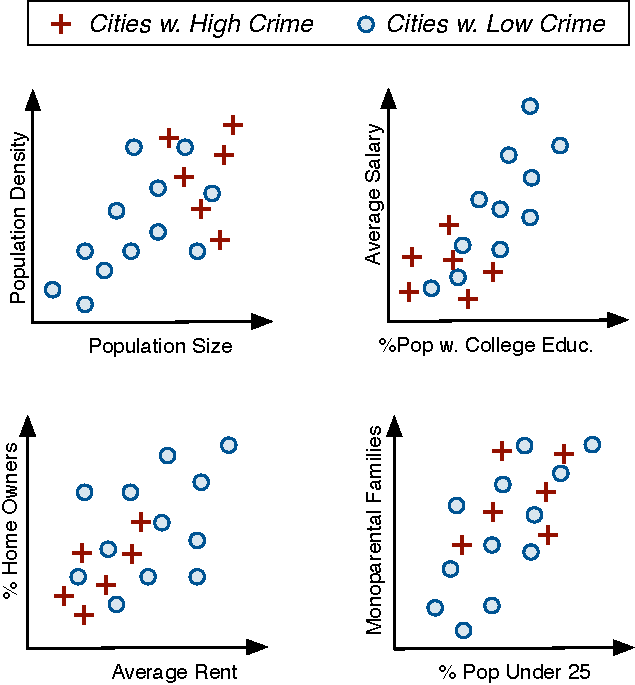
\includegraphics[width=.8\columnwidth]{Images/CharacViews} \caption{Four
    examples of characteristic views.} \label{fig:characteristic-views}
\end{figure}


\section{Problem Formulation}
\label{sec:algorithm}

We described the intuition behind characteristic views.  We now formalize the
problem. We present Ziggy's objective function, and we describe how it scores
the views.

\subsection{General Statement} 
When seeking views, Ziggy must consider three aspects. It must first find
columns on which the users' selection have an ``unusual'' statistical
distribution.  Thereafter, it must enforce that its views are coherent (i.e.,
they describe the same aspect of the data) and that they are diverse.  Let us
formalize those objectives.

\label{sec:problem}
Let the random variables $C_1, \ldots, C_M$ represent the co\-lumns in the
database.  We assume that the variable $C_k^I$ represent the tuples covered by
the user's query and that $C_k^O$ represents the tuples outside the selection,
as shown in Figure~\ref{fig:setting}.  Ziggy's aim is to find a set of at most
$D$ columns such that the distribution of $C_1^O, \ldots, C_D^O$ is as
different as possible from that of $C_1^I, \ldots, C_D^I$. If $\mathfrak{D}$
represents a measure of distribution divergence from the statistics literature,
our aim is to find the views $\mathcal{V}_i = \{C_1, \ldots, C_D\}$ that
maximize the following quantity:
\begin{equation}
    \label{eq:objective0}
    \textsc{score} (\mathcal{V}_i) = \mathfrak{D}\big( C_1^O, \ldots, C_D^O \,;\,
        C_1^I, \ldots, C_D^I \big)\\
\end{equation}
Common examples of divergence functions $\mathfrak{D}$ are the distance between
the centroids and the Kullback-Leibler divergence~\cite{wasserman2013all}.  We
will present our own in the next subsection.

\begin{figure}[t!]
    \centering
    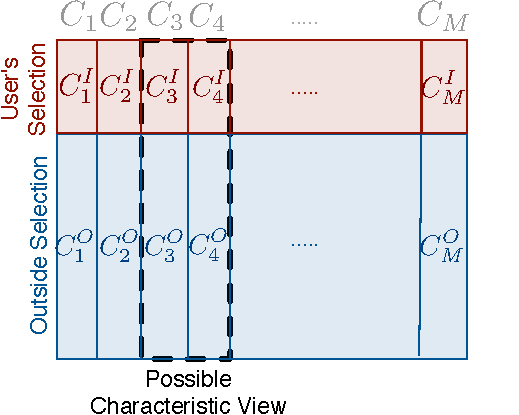
\includegraphics[width=.7\columnwidth]{Images/Setting}
    \caption{Our problem setting.}
    \label{fig:setting}
\end{figure}
Equation~\ref{eq:objective0} is not complete because it favors large,
he\-terogeneous subspaces.  For many functions $\mathfrak{D}$, $\textsc{score}
(\mathcal{V}_i)$ reaches its maximal when $\mathcal{V}_i$ contains all the
columns in the database. Furthermore, maximizing $\textsc{score}
(\mathcal{V}_i)$ alone does not guarantee that the variables are thematically
related. To obtain smaller, more homogeneous subspaces, we introduce a
constraint. Let $\mathfrak{S}$ describe a measure of statistical dependency,
such as  the correlation or the mutual information~\cite{wasserman2013all}. The
\emph{tightness} of a view measures how interdependent its variables are:
\begin{equation}
    \textsc{tightness}(\mathcal{V}_i) = \min_{C_k,C_l \in \mathcal{V}_i}\;
    \mathfrak{S}(C_k, C_l) 
\end{equation}
We introduce a constraint $\mathit{MIN}_{tight}$ on this quantity:
\begin{equation}
    \textsc{tightness}(\mathcal{V}_i) \geq \mathit{MIN}_{tight}
\end{equation}
%Another shortcoming of the objective function exposed in
%Equation~\ref{eq:objective0} is that it leads to redundancy. A small number of
%columns may appear in all the best views. To control this effect, we introduce
%a second constraint.  Assume that we have already discovered $i-1$ views
%$\mathcal{V}_1, \ldots, \mathcal{V}_{i-1}$. Let the notation $\mathcal{V}_{1
%\ldots i-1}$ describe their union, i.e., $\mathcal{V}_{1 \ldots i-1} =
%\bigcup_{v \in [1,i-1]} \mathcal{V}_v$.  We set a higher limit on
%the number of columns present in both $\mathcal{V}_i$ and $\mathcal{V}_{1\ldots
%i-1}$, that is:
%\begin{equation}
%    \text{overlap}(\mathcal{V}_{1 \ldots i-1}, \mathcal{V}_i) =  
%    \left|\mathcal{V}_{1\ldots i-1} \cap  \mathcal{V}_i \right|
%\end{equation}
%We can now present our full problem. 
%
%\begin{problem}
%Assume that we have already discovered $i-1$ views. Given 
%the parameters $MIN_{tightness}$ and $MAX_{overlap}$, our aim is
%to find a view $\mathcal{V}_i$ which is not included in a previous view and
%that solves the following optimization problem:
%\begin{equation}
%    \label{eq:objective}
%    \begin{aligned}
%        \text{Argmax}_{\mathcal{V}_i}\; 
%        & \text{score} (\mathcal{V}_i)\\
%         \text{s.t.  } 
%%         & \mathcal{V}_i \not\subset \mathcal{V}_v\text{, for } v \in [1, i-1]\\
%         &\text{tightness}(\mathcal{V}_i) \geq MIN_{tightness}\\ 
%         &\text{overlap}(\mathcal{V}_{1 \ldots i-1}, \mathcal{V}_i) \leq MAX_{overlap}
%    \end{aligned}
%\end{equation}
%\end{problem}
Another shortcoming of the objective function exposed in
Equation~\ref{eq:objective0} is that it leads to redundancy.  Typically, the
results will contain every possible subsets of a few dominant variables. To
keep the output short and diverse, we enforce that the view are disjoint.
Assume that we have already discovered $i-1$ views $\mathcal{V}_1, \ldots,
\mathcal{V}_{i-1}$, and that we are seeking a new view $\mathcal{V}_i$. Let the
notation $\mathcal{V}_{1 \ldots i-1}$ describe the union
$\mathcal{V}_{1 \ldots i-1} = \bigcup_{v \in [1,i-1]} \mathcal{V}_v$.  We
introduce the following constraint:
\begin{equation}
    \textsc{overlap}(\mathcal{V}_{1\ldots i-1},\mathcal{V}_i) = 
        \left| \mathcal{V}_{1\ldots i-1} \cap  \mathcal{V}_i \right| = 0
\end{equation}
We can now present our full problem. 

\begin{problem}
    Assume that we have already discovered $i-1$ views. If $\mathit{MIN}_{tight}$
describes a user-defined parameter, our aim is to find a view $\mathcal{V}_i$
that solves the following system:
\begin{equation}
    \label{eq:objective}
    \begin{aligned}
        \text{Argmax}_{\mathcal{V}_i}\; 
        & \textsc{score} (\mathcal{V}_i)\\
         \text{s.t.  } 
%         & \mathcal{V}_i \not\subset \mathcal{V}_v\text{, for } v \in [1, i-1]\\
         &\textsc{tightness}(\mathcal{V}_i) \geq \mathit{MIN}_{tight}\\ 
         &\textsc{overlap}(\mathcal{V}_{1\ldots i-1},\mathcal{V}_i) = 0\\
%         &\text{overlap}(\mathcal{V}_{1 \ldots i-1}, \mathcal{V}_i) \leq MAX_{overlap}
    \end{aligned}
\end{equation}
\end{problem}

\subsection{Dissimilarity Measure}
The statistics literature presents many options to instantiate the statistical 
divergence measure $\mathfrak{D}$~\cite{wasserman2013all}. But most of these
operate in a ``black box'' fashion: they indicate how much two distributions
differ, but they do not explain why. We now introduce our own function, the
\emph{Zig-Dissimilarity}, that overcomes this problem.
\pagebreak

\begin{figure}[t!]
    \centering
    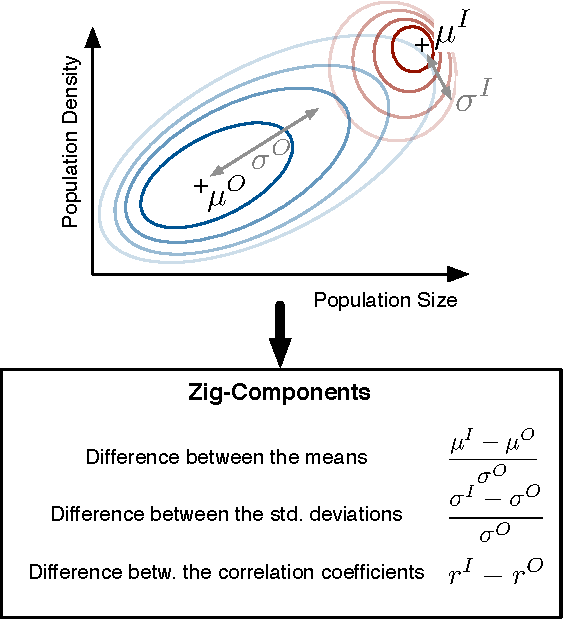
\includegraphics[width=.8\columnwidth]{Images/Zig-Dissimilarity}
    \caption{Examples of Zig-Components.}
    \label{fig:zig-dissim}
\end{figure}

The idea behind the Zig-Dissimilarity is to compute se\-veral simple
indicators of dissimilarity, the \emph{Zig-Components}, and aggregate them into
one synthetic score.  Figure~\ref{fig:zig-dissim} pre\-sents three such
indicators: the difference between the means, the difference between the
standard deviations and the difference between the correlation coefficients. We
see that each Zig-Component highlights one particular aspect of the
difference between the distributions.  Also, these functions are verifiable:
the users can inspect the charts and check whether they hold.  Most of our
Zig-Components come from the statistics literature, where they are referred to
as \emph{effect sizes}~\cite{hedges2014statistical}. Observe that we test
dissimilarities in spaces with one but also two dimensions. For instance, the
difference between the correlation coefficients involves two columns. In
principle, we could design Zig-Components for higher dimensionalities.
Nevertheless, those only add marginal accuracy gains  in practice, at the cost
of significant processing times. We refer the interested reader to our full
paper for other examples of Zig-Components (e.g., involving categorical data).

To aggregate the Zig-Components, we normalize them and compute a weighted sum.
The normalization enforces that the indicators have comparable scale. The
weights in the final sum are defined by the user. Thanks to this mechanism, our
explorers can express their preference for one type of difference over the
others. 

The advantage of our divergence measure is that it lets Ziggy \emph{explain}
its choices. To illustrate, let us return to the first view of
Figure~\ref{fig:characteristic-views}. A classic subspace search algorithm
would present the chart without further explanations. In contrast, our system
can motivate its decisions. In this case, it comments the view as follows:
\begin{quotation}
    ``On the columns~\texttt{Population} and \texttt{Density}, your selection has
    particularly high values and a low variance''
\end{quotation} 
This short sentence describes why Ziggy chose the columns \texttt{Population}
and \texttt{Density}. The users can interpret these explanations as hints for
further exploration, to make sure that they have not missed any 
aspect of their query results.

\section{Ziggy's Architecture}
\label{sec:solution}

%We formalized the multi-view characterization problem. We now present how Ziggy
%solves it.
We now present how Ziggy solves the tuple characterization problem.
Figure~\ref{fig:architecture} presents Ziggy's tuples description pipeline.  It
includes three stages: preparation, view search and post-processing.
During the preparation stage, Ziggy collects the statistics necessary to build
the views. In the view search stage, it effectively forms the views.
During the last step, it checks if those views are statistically robust and it
generates the explanations.

\begin{figure}[t!]
    \centering
    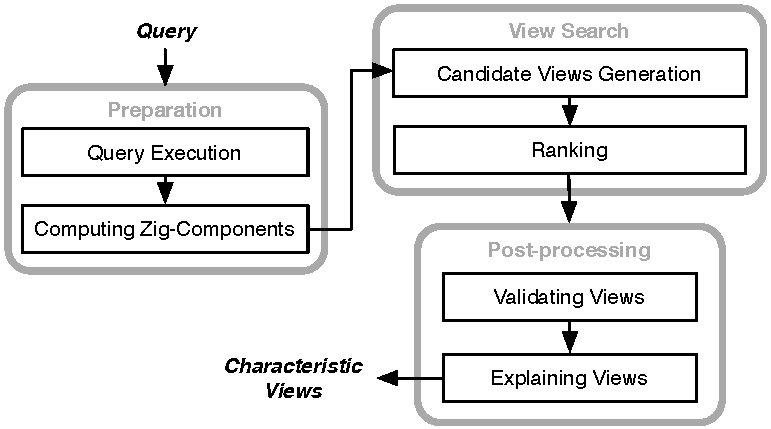
\includegraphics[width=\columnwidth]{Images/Algorithm}
    \caption{Ziggy's Tuples Description Pipeline.}
    \label{fig:architecture}
\end{figure}
\textbf{Preparation.} During the preparation step, Ziggy executes the user's
query, loads the results, and computes the Zig-Components associated to each
column and each couple of columns. This is often the most time consuming step.
In our full paper, we present a strategy to share computations between queries,
and therefore reduce the amount of data to read. The output of these operations
is a table, which describes the Zig-Components associated to each variable and
each pair of variables.

\textbf{View Search.} During this step, Ziggy builds the views. It operates as
follows. First, it enumerates the groups of columns which satisfy the
constraints of Equation~\ref{eq:objective}.  It does so with a graph-based
algorithm: it materializes the graph formed by the column's pairwise
dependencies, and partitions it with a clique search or clustering algorithm.
In our implementation, we used complete linkage
clustering~\cite{wasserman2013all}. This method is simple, well established,
and it provides a dendrogram, i.e.,  visual support to help setting the
parameter $\mathit{MAX}_{tight}$.  From this step, Ziggy obtains a set of candidate
views.  It scores them using the Zig-Components obtained previously, and it
ranks the set accordingly.
\begin{figure*}[!th]
    \centering
    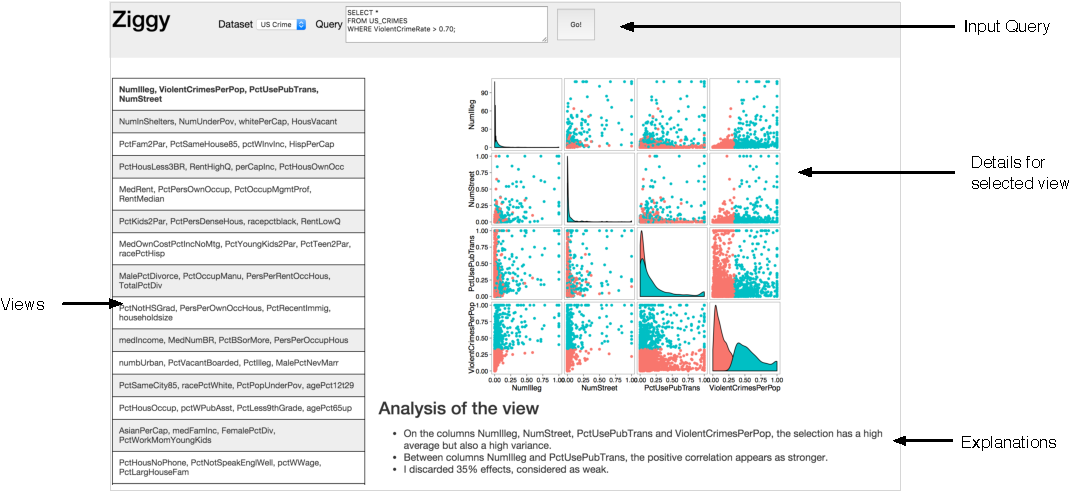
\includegraphics[width=.96\textwidth]{Images/ScreenDetail}
    \caption{Snapshot of Ziggy's interface.}
    \label{fig:screenshot}
\end{figure*}


\textbf{Post-Processing.} During the final phase, Ziggy evaluates the
statistical robustness of the views. The aim is to control spurious findings,
that is, differences caused by chance. For each view, it tests the
significance of the Zig-Component separately, using asymptotic bounds from the
literature~\cite{hedges2014statistical}. Then it aggregates the confidence
scores associated with each component. Depending on the users' preferences, it
retains the lowest value, or it uses more advanced aggregation schemes such
as the Bonferroni correction~\cite{wasserman2013all}. 

During the last step, Ziggy also generates the explanations. Given the
composite nature of the Zig-Dissimilarity, this step is straightforward: Ziggy
choses the Zig-Components associated with the highest levels of confidence, and
it describes them with text. We implemented the text generation functionalities
with handwritten rules and  regular expressions.

\pagebreak



\section{Implementation and Demo}
\label{sec:demo}

\subsection{Overview of the System}
\label{sec:archi}
Our demonstration system comprises three components. In the bottom layer, a
DBMS stores and delivers the data (we chose MonetDB). The middle layer
comprises the query characterization engine and a Web server. We developed both
components in R, except for a few critical performance operations written in C (those
related to computing Zig-Components). The Web server relies on the package
\texttt{Shiny}. The front-end is based on HTML and Javascript. 

Figure~\ref{fig:screenshot} presents a snapshot of our demonstration system.
Users specify their queries in the text box of the top panel. Ziggy returns the
views on the left side, ranked by decreasing order of dissimilarity.  It
displays the explanations on the right side.

\subsection{Use Cases}
\label{sec:usecases}

We will demonstrate Ziggy with three real-life datasets.
\begin{itemize0}
    \item The \textbf{Box Office} dataset describes Hollywood movies released
        between 2007 and 2013. We will use it to introduce the main concepts behind
        Ziggy: the query description problem, how Ziggy choses views and how to
        read them. The data contains 900 tuples and 12 columns.
    \item The \textbf{US Crime} database contains 128 crime and socio-economic
        indicators for 1994 US Cities. The dataset is freely available on the
        UCI Repository\footnote{\url{https://archive.ics.uci.edu/ml/datasets/Communities+and+Crime}}.
        The use case is similar to the running example used throughout this
        paper. We hope to surprise our visitors by showing that seemingly
        superfluous variables can have a strong predictive power - such as the
        number of boarded windows in a given neighborhood.
    \item The \textbf{Countries and Innovation} dataset describes innovation
        and patents for different regions of the world. We obtained it by
        combining different tables from the Website of the OECD, an international
        economic organization\footnote{\url{http://stats.oecd.org/}}. It
        contains 6,823 rows and 519 columns. We will show that Ziggy can
        highlight complex phenomena, in effect generating hypotheses for future
        exploration.
\end{itemize0}
During our presentation, we will use ready-made queries and encourage the
visitors to suggest their own.

\section{Conclusion}
\label{sec:conclusion}
During the last few years, authors have introduced dozens of methods to
discover new, interesting queries. In this paper, we tackled the complementary
problem: once our users have a query, how do they know if it is a good one?
Our short term objective is to demonstrate Ziggy and let visitors challenge our
system. On the long term, we intend to distribute our tuple description engine
as a library, to be included into external exploration systems.

